\chapter{CDCL}
\emph{Conflict-driven clause learning} (CDCL) ist ein Ansatz, um SAT-Probleme effizient zu lösen.
Die in diesem Kapitel vorgestellen Informationen stammen aus dem Buch \emph{The Art of Computer Programming, Volume 4, Fascicle 6: Satisfiability}~\cite{The_Art_of_Computer_Programming_Volume_4_Fascicle_6_Satisfiability}
Im Allgemeinen funktionieren SAT-Solver so, dass sie jede Möglichkeit ausprobieren.
Dies lässt sich als Baum darstellen (siehe~\cref{fig:sat_tree}).
\begin{figure}[ht]
	\centering
	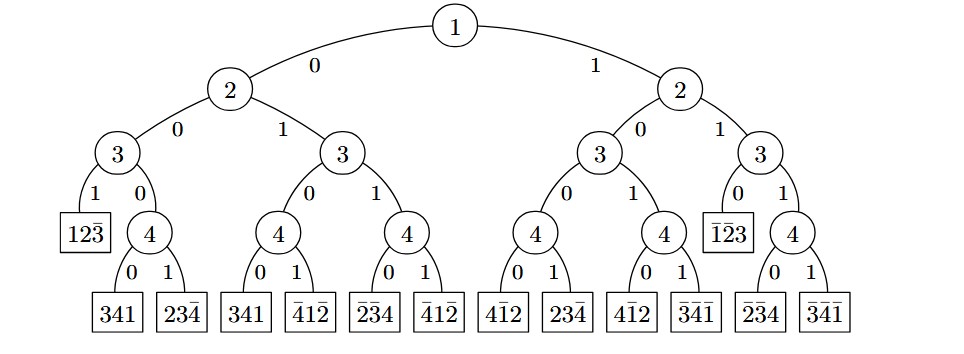
\includegraphics[width=1\linewidth]{figures/sat_tree.png}
	\caption{Ein Baum welcher die Möglichen Entscheidungen eines SAT-Solvers darstellt. Jeder Ast entspricht Belegungen der Literale}
	\label{fig:sat_tree}
\end{figure}
Das Besondere am CDCL-Ansatz ist, dass nicht die Äste iterativ abgearbeitet werden, sondern dass es einen Pfad gibt.
Der Pfad ist eine aktuelle Teilbelegung der Literale. Theoretisch entspricht dies einem Ast im Baum, aber die Auswahl der Belegung basiert nicht direkt auf dem Baum.
Für jedes belegte Literal muss eine Begründung angegeben werden. Diese Begründungen werden bei Konflikten relevant.

\section{\emph{Unit-Klauseln}}
Der Grundansatz zur Erweiterung des Pfades besteht darin, \emph{Unit-Klauseln} zu finden.
Das sind Klauseln, in denen nur ein Literal noch nicht belegt ist und die Klausel nicht erfüllt ist.
Zum Beispiel kann durch die Klausel \((\overline{x_1} \lor x_2 \lor \overline{x_3})\) und den Pfad \((\overline{x_2}, x_3)\) das Literal \(\overline{x_1}\) dem Pfad hinzugefügt werden. Die Klausel dient dabei als Begründung.
% TODO eventuell ergänzen, dass immer nur zwei Literale betrachtet werden

Sollten keine weiteren \emph{Unit-Klauseln} existieren, wird basierend auf Heuristiken ein Literal belegt.
Bei dieser Art der Belegung wird intern vermerkt, dass eine neue Entscheidungsebene erreicht wurde.
Die Entscheidungsebenen werden auch bei Konflikten wichtig. Es ist zu beachten, dass jeder Abschnitt des Pfades einer Entscheidungsebene zugeordnet werden kann.
Ein Literal, das weiter rechts im Pfad steht, wird einer höheren Entscheidungsebene zugeordnet.

\section{Konflikte}
Ein Konflikt tritt auf, wenn ein Literal zum zweiten Mal dem Pfad hinzugefügt werden soll, das Literal aber bereits eine andere Belegung besitzt.
Hier zeigt sich der besondere Ansatz von CDCL.
Kommt es zu einem Konflikt, wird nicht einfach zu einer vorherigen Entscheidungsebene zurückgekehrt. Stattdessen werden die Informationen, wie es zu dem Konflikt kam, genutzt.
Sei
\[
c = (\overline{l} \lor \overline{a_1} \lor \ldots \lor \overline{a_k})
\]
eine Klausel, die einen Konflikt aufweist. Das bedeutet, alle Literale wurden dem Pfad hinzugefügt und die Klausel ist nicht erfüllt.

Es kann angenommen werden, dass \(l\) und ein weiteres Literal \(a_i\) aus \(c\) auf der höchsten Entscheidungsebene \(d\) liegen.
Andernfalls wäre \(c\) eine \emph{Unit-Klausel} und somit wäre \(l\) bereits auf \(d-1\) belegt worden.
Weiterhin kann angenommen werden, dass das Literal \(l\) das rechteste Literal von allen Literalen aus \(c\) im Pfad ist. Also das Literal aus \(c\), das zuletzt belegt wurde.
Daraus folgt, dass \(l\) keine neue Entscheidungsebene erzeugt hat, da zumindest \(a_i\) vor \(l\) auf der Entscheidungsebene \(d\) belegt wurde.

Es existiert somit eine Begründung
\[
(\overline{l} \lor \overline{r_1} \lor \ldots \lor \overline{r_k})
\]
für die Belegung von \(l\).
Damit kann folgende Klausel erzeugt werden
\[
c' = (\overline{a_1} \lor \ldots \lor \overline{a_k} \lor \overline{r_1} \lor \ldots \lor \overline{r_k})
\]
obei \(c'\) mindestens eine Belegung aus der Entscheidungsebene \(d\) enthält.
Sollte es ein weiteres Literal außer \(a_i\) geben, das auf der Entscheidungsebene \(d\) belegt wurde, ist \(c'\) ebenfalls eine Konfliktklausel.
In diesem Fall wird \(c'\) rekursiv so lange erzeugt bis es genau ein Literal \(\overline{x}\) gibt, das auf Entscheidungsebene \(d\) belegt wurde.
Der rekursive Aufruf fügt dabei die Begründung des zweiten Literals aus Entscheidungsebene \(d\) ohne dieses Literal zu \(c'\) hinzu.
Von den restlichen Literalen in \(c'\) wird dann die höchste Entscheidungsebene bestimmt und zu dieser zurückgekehrt.
Anschließend wird \(\overline{x}\) dem aktuellen Pfad hinzugefügt und \(c'\) als Begründung für die Belegung verwendet.
% TODO als Bild veranschaulichen? keine Idee wie

% TODO Gelernte Klauseln reduzieren vermutlich nicht relevant
% TODO Pfa4d zurücksetzen ohne Konflikt vermutlich nicht relevant

\section{\emph{Propagation}}
Der CDCL Solver namens \emph{CaDiCaL}~\cite{cadical} von Armin Biere ermöglicht es, eine neue Entscheidungsebene mit einer eigenen Funktion zu erzeugen.
Diese Funktion kann dann das nächste Literal setzen.
Im Folgenden wird diese Funktion \emph{Propagation} genannt.
Die Idee bei dieser \emph{Propagation} ist es, die Bedingungen aus~\cref{sec:exclude_edges} auf Teilinstanzen anzuwenden.

\subsection{Visualisierung}
Der erste Schritt war es, die Teilinstanzen, mit denen die \emph{Propagation} aufgerufen wird, zu visualisieren.
\begin{figure}[htb]
    \centering
    
\includegraphics[width=1\linewidth]{cdcl/propergation.pdf}
    \caption{Eine Teilinstanz bei einem \emph{Propagation} Aufruf. Blau auf false gesetzt, grün auf true. Grüner Knoten Sollgrad erfüllt. Zahl in Knoten ist Sollgrad.
	TODO schön aufschreiben mit finalem Bild und erklären das von rand ausgehend fertig}
    \label{fig:cdcl:propagation}
\end{figure}
In~\cref{fig:cdcl:propagation} ist eine beispielhafte Teilinstanz dargestellt.
Bei der Visualisierung ist aufgefallen, dass oft vom Rand ausgehend die Instanz gelöst wurde, also es meistens einen \emph{Arm} gab, welcher in die Mitte der Instanz reichte.
Selten gab es einzelne Konstrukte in der Mitte der Instanz mit keinen Verbindungen zum Rand.

\subsection{Implementierung}
Die Idee der \emph{Propagation} ist es, die Bedingungen aus~\cref{sec:exclude_edges} zum Halbieren der Instanz zu verwenden.
Der Vorteil an den Teilinstanzen ist, dass der \emph{Arm} die Instanz meist schon irgendwo zum Teil halbiert.
Es können also Kanten getestet werden, welche die Halbierung abschließen.
Dafür wird mit einem Arrangement verfolgt, welche Kanten aktiv sind.
Es muss nur darauf geachtet werden, dass bei jeder neuen Entscheidungsebene das Arrangement gespeichert und einer Ebene zugeordnet wird.
Sollte es zu einem Konflikt kommen, wird das Arrangement zu der richtigen Entscheidungsebene zurückgesetzt.
Wenn die \emph{Propagation} aufgerufen wird, können alle Faces des Arrangements betrachtet werden.
Hierbei sind nur Faces relevant, welche mehr als drei Kanten haben.
Bei diesen können alle Teilenden Kanten erzeugt werden, indem alle Zweierkombinationen der Randknoten des Faces betrachtet werden.
Dadurch wird das Face in zwei Hälften geteilt und die Kante zwischen den Knoten der Zweierkombination kann getestet werden.
Sollte die Kante zu einem Konflikt führen, kann das zugehörige Literal \(l\) auf \emph{falsch} gesetzt werden.
Als Begründung kann folgende Klausel verwendet werden:
\[
(\overline{l} \lor \bigvee_{e \in E_A}\overline{x_e})
\]
Wobei \(E_A\) die Menge der aktiven Kanten ist.